\chapter{Score-based Pullback Riemannian Geometry}
\section{Proof of \ref{thm:rae-error}}
\label{app:proof-of-rae-error}

\paragraph{Auxiliary lemma}

\begin{lemma}
    \label{lem:rae-bound-phi-metric}
        Let $\diffeo:\Real^\dimInd \to \Real^\dimInd$ be a smooth diffeomorphism and let $\stroco: \Real^\dimInd \to \Real$ be a quadratic function of the form \ref{eq:quadratic-stroco} with diagonal $\spdMatrix \in \Real^{\dimInd\times \dimInd}$. Furthermore, let $\density:\Real^\dimInd \to\Real$ be the corresponding probability density of the form \ref{eq:stroco-diffeo-density}. Finally, consider $\RAErelerror\in [0,1]$ and the mappings $\RAEencoder_\RAErelerror:\Real^\dimInd \to \Real^{\dimInd_\RAErelerror}$ and $\RAEdecoder_\RAErelerror:\Real^{\dimInd_\RAErelerror} \to \Real^\dimInd$ in \ref{eq:rae-encoder},\ref{eq:rae-decoder} with $\dimInd_\RAErelerror \in [\dimInd]$ as in \ref{eq:dimind-epsilon}.
    
        Then, for any $\RAEboundParamB \in [0,1)$ and any $\RAEboundParam\in [0,1- \RAEboundParamB)$
        \begin{equation}
        \mathbb{E}_{\stoVector \sim \density}[\distance_{\Real^{\dimInd}}^\diffeo (D_\RAErelerror(E_\RAErelerror(\stoVector)), \stoVector)^2 e^{\frac{\RAEboundParamB}{2} \diffeo(\stoVector)^\top \spdMatrix^{-1} \diffeo(\stoVector)}] \leq \RAErelerror \frac{\RAEdiffeoRegConstant \RAEinvdiffeoRegConstant}{1 - \RAEboundParamB - \RAEboundParam} \Bigl(\frac{1 + \RAEboundParam}{1 - \RAEboundParamB - \RAEboundParam} \Bigr)^{\frac{\dimInd}{2}} \sum_{\sumIndA=1}^{\dimInd} \spdMatrixDiag_{\sumIndA},
        \label{eq:lem-rae-bound}
\end{equation}
where
\begin{equation}
    \RAEinvdiffeoRegConstant := \sup_{\Vector\in \Real^{\dimInd}} \{ |\det (D_{\diffeo(\Vector)} \diffeo^{-1})| e^{-\frac{\RAEboundParam}{2} \diffeo(\Vector)^\top \spdMatrix^{-1} \diffeo(\Vector) } \},
    \label{eq:RAEinvdiffeoRegConstant}
\end{equation}
and
\begin{equation}
    \RAEdiffeoRegConstant := \sup_{\Vector\in \Real^{\dimInd}} \{ |\det (D_{\Vector} \diffeo)| e^{-\frac{\RAEboundParam}{2} \diffeo(\Vector)^\top \spdMatrix^{-1} \diffeo(\Vector) } \}.
    \label{eq:RAEdiffeoRegConstant}
\end{equation}
\end{lemma}

\begin{proof}
    We need to distinct two cases: (i) $\dimInd_\RAErelerror = \dimInd$ and (ii) $1 \leq \dimInd_\RAErelerror < \dimInd$

    (i) If $\dimInd_\RAErelerror = \dimInd$ we have that $D_\RAErelerror(E_\RAErelerror(\Vector)) = \Vector$ for any $\Vector\in \Real^\dimInd$. In other words
    \begin{equation}
        \mathbb{E}_{\stoVector \sim \density}[\distance_{\Real^{\dimInd}}^\diffeo (D_\RAErelerror(E_\RAErelerror(\stoVector)), \stoVector)^2 e^{\frac{\RAEboundParamB}{2} \diffeo(\stoVector)^\top \spdMatrix^{-1} \diffeo(\stoVector)}] = 0 \leq \RAErelerror \frac{\RAEdiffeoRegConstant \RAEinvdiffeoRegConstant}{1 - \RAEboundParamB - \RAEboundParam} \Bigl(\frac{1 + \RAEboundParam}{1 - \RAEboundParamB - \RAEboundParam} \Bigr)^{\frac{\dimInd}{2}} \sum_{\sumIndA=1}^{\dimInd} \spdMatrixDiag_{\sumIndA}.
    \end{equation}

    (ii) Next, we consider the case $1 \leq \dimInd_\RAErelerror < \dimInd$.
    First, notice that we can rewrite 
    \begin{multline}
        \| \diffeo(D_\RAErelerror(E_\RAErelerror(\Vector))) - \diffeo(\Vector) \|_2^2 \overset{\text{\ref{eq:rae-encoder,eq:rae-decoder}}}{=} \|\sum_{\sumIndC=1}^{\dimInd_\RAErelerror} (\diffeo(\Vector), \mathbf{e}^{\sumIndA_\sumIndC})_2 \mathbf{e}^{\sumIndA_\sumIndC} - \diffeo(\Vector)\|_2^2 = \|\sum_{\sumIndC=\dimInd_\RAErelerror+1}^{\dimInd} (\diffeo(\Vector), \mathbf{e}^{\sumIndA_\sumIndC})_2 \mathbf{e}^{\sumIndA_\sumIndC}\|_2^2 \\
        \overset{\text{orthogonality}}{=} \sum_{\sumIndC=\dimInd_\RAErelerror+1}^{\dimInd} \|(\diffeo(\Vector), \mathbf{e}^{\sumIndA_\sumIndC})_2 \mathbf{e}^{\sumIndA_\sumIndC}\|_2^2 = \sum_{\sumIndC=\dimInd_\RAErelerror+1}^{\dimInd}(\diffeo(\Vector), \mathbf{e}^{\sumIndA_\sumIndC})_2^2 = \sum_{\sumIndC=\dimInd_\RAErelerror+1}^{\dimInd}\diffeo(\Vector)_{\sumIndA_\sumIndC}^2.
        \label{eq:rewrite-RAEx-x}
    \end{multline}
    Moreover, we define
    \begin{equation}
        \RAEnormalizationConstant :=  \int_{\Real^{\dimInd}} e^{-\frac{1}{2} \diffeo(\Vector)^\top \spdMatrix^{-1} \diffeo(\Vector)} \mathrm{d} \Vector.
        \label{eq:RAEnormalizationConstant}
    \end{equation}
    
    Then, 
    \begin{multline}
        \mathbb{E}_{\stoVector \sim p}[\distance_{\Real^{\dimInd}}^\diffeo (D_\RAErelerror(E_\RAErelerror(\stoVector)), \stoVector)^2 e^{\frac{\RAEboundParamB}{2} \diffeo(\stoVector)^\top \spdMatrix^{-1} \diffeo(\stoVector)}] = \frac{\int_{\Real^\dimInd}  \| \diffeo(D_\RAErelerror(E_\RAErelerror(\Vector))) - \diffeo(\Vector) \|_2^2 e^{-(\frac{1}{2} - \frac{\RAEboundParamB}{2}) \diffeo(\Vector)^\top \spdMatrix^{-1} \diffeo(\Vector)} \mathrm{d} \Vector}{\int_{\Real^{\dimInd}} e^{-\frac{1}{2} \diffeo(\Vector)^\top \spdMatrix^{-1} \diffeo(\Vector)} \mathrm{d} \Vector}  \\
        \overset{\text{\ref{eq:RAEnormalizationConstant}}}{=} \frac{1}{\RAEnormalizationConstant} \int_{\Real^\dimInd}  \| \diffeo(D_\RAErelerror(E_\RAErelerror(\Vector))) - \diffeo(\Vector) \|_2^2 e^{-(\frac{1}{2} - \frac{\RAEboundParamB}{2}) \diffeo(\Vector)^\top \spdMatrix^{-1} \diffeo(\Vector)} \mathrm{d} \Vector \\
        \overset{\text{\ref{eq:rewrite-RAEx-x}}}{=} \frac{1}{\RAEnormalizationConstant} \int_{\Real^\dimInd}  \sum_{\sumIndC=\dimInd_\RAErelerror+1}^{\dimInd}\diffeo(\Vector)_{\sumIndA_\sumIndC}^2 e^{-(\frac{1}{2} - \frac{\RAEboundParamB}{2}) \diffeo(\Vector)^\top \spdMatrix^{-1} \diffeo(\Vector)} \mathrm{d} \Vector = \frac{1}{\RAEnormalizationConstant} \sum_{\sumIndC=\dimInd_\RAErelerror+1}^{\dimInd} \int_{\Real^\dimInd}  \diffeo(\Vector)_{\sumIndA_\sumIndC}^2 e^{-(\frac{1}{2} - \frac{\RAEboundParamB}{2}) \diffeo(\Vector)^\top \spdMatrix^{-1} \diffeo(\Vector)} \mathrm{d} \Vector\\
        \overset{\Vector =\diffeo^{-1}(\VectorB) }{=} \frac{1}{\RAEnormalizationConstant} \sum_{\sumIndC=\dimInd_\RAErelerror+1}^{\dimInd} \int_{\Real^\dimInd} \VectorB_{\sumIndA_\sumIndC}^2 e^{-(\frac{1}{2} - \frac{\RAEboundParamB}{2}) \VectorB^\top \spdMatrix^{-1} \VectorB} |\det(D_{\VectorB}\diffeo^{-1})|\mathrm{d} \VectorB \\
        = \frac{1}{\RAEnormalizationConstant} \sum_{\sumIndC=\dimInd_\RAErelerror+1}^{\dimInd} \int_{\Real^\dimInd} \VectorB_{\sumIndA_\sumIndC}^2 e^{-(\frac{1}{2} - \frac{\RAEboundParamB}{2} - \frac{\RAEboundParam}{2}) \VectorB^\top \spdMatrix^{-1} \VectorB} |\det(D_{\VectorB}\diffeo^{-1})|  e^{-\frac{\RAEboundParam}{2} \VectorB^\top \spdMatrix^{-1} \VectorB}\mathrm{d} \VectorB\\
        \leq \frac{\sup_{\VectorB\in \Real^\dimInd} \{|\det(D_{\VectorB}\diffeo^{-1})|  e^{-\frac{\RAEboundParam}{2} \VectorB^\top \spdMatrix^{-1} \VectorB}\}}{\RAEnormalizationConstant} \sum_{\sumIndC=\dimInd_\RAErelerror+1}^{\dimInd} \int_{\Real^\dimInd} \VectorB_{\sumIndA_\sumIndC}^2 e^{-(\frac{1}{2} - \frac{\RAEboundParamB}{2} - \frac{\RAEboundParam}{2}) \VectorB^\top \spdMatrix^{-1} \VectorB} \mathrm{d} \VectorB \\
        \overset{\text{\ref{eq:RAEinvdiffeoRegConstant}}}{=} \frac{\RAEdiffeoRegConstant}{\RAEnormalizationConstant} \sum_{\sumIndC=\dimInd_\RAErelerror+1}^{\dimInd} \int_{\Real^\dimInd} \VectorB_{\sumIndA_\sumIndC}^2 e^{-(\frac{1}{2} - \frac{\RAEboundParamB}{2} - \frac{\RAEboundParam}{2}) \VectorB^\top \spdMatrix^{-1} \VectorB} \mathrm{d} \VectorB = \frac{\RAEdiffeoRegConstant}{\RAEnormalizationConstant} \sum_{\sumIndC=\dimInd_\RAErelerror+1}^{\dimInd} \int_{\Real^\dimInd} \VectorB_{\sumIndA_\sumIndC}^2 e^{-(\frac{1}{2} - \frac{\RAEboundParamB}{2} - \frac{\RAEboundParam}{2}) \sum_{\sumIndB=1}^\dimInd  \frac{\VectorB_\sumIndB^2}{\spdMatrixDiag_{\sumIndB}} } \mathrm{d} \VectorB  \\
        = \frac{\RAEdiffeoRegConstant}{\RAEnormalizationConstant} \sum_{\sumIndC=\dimInd_\RAErelerror+1}^{\dimInd} \int_{\Real} \VectorB_{\sumIndA_\sumIndC}^2 e^{-(\frac{1}{2} - \frac{\RAEboundParamB}{2} - \frac{\RAEboundParam}{2})  \frac{\VectorB^2}{\spdMatrixDiag_{\sumIndA_\sumIndC}} } \mathrm{d} \VectorB_{\sumIndA_\sumIndC} \int_{\Real^{\dimInd-1}} e^{-(\frac{1}{2} - \frac{\RAEboundParamB}{2} - \frac{\RAEboundParam}{2}) \sum_{\sumIndB\neq \sumIndA_\sumIndC}^\dimInd  \frac{\VectorB_\sumIndB^2}{\spdMatrixDiag_{\sumIndB}} } \mathrm{d} \VectorB_{1} \ldots \mathrm{d} \VectorB_{\sumIndA_\sumIndC -1} \mathrm{d} \VectorB_{\sumIndA_\sumIndC +1} \ldots \mathrm{d} \VectorB_{\dimInd}\\
        = \frac{\RAEdiffeoRegConstant}{\RAEnormalizationConstant} \sum_{\sumIndC=\dimInd_\RAErelerror+1}^{\dimInd} \frac{\spdMatrixDiag_{\sumIndA_\sumIndC}}{(1 - \RAEboundParamB - \RAEboundParam)} \int_{\Real}  e^{-(\frac{1}{2} - \frac{\RAEboundParamB}{2} - \frac{\RAEboundParam}{2})  \frac{\VectorB^2}{\spdMatrixDiag_{\sumIndA_\sumIndC}} } \mathrm{d} \VectorB_{\sumIndA_\sumIndC} \int_{\Real^{\dimInd-1}} e^{-(\frac{1}{2} - \frac{\RAEboundParamB}{2} - \frac{\RAEboundParam}{2}) \sum_{\sumIndB\neq \sumIndA_\sumIndC}^\dimInd  \frac{\VectorB_\sumIndB^2}{\spdMatrixDiag_{\sumIndB}}} \mathrm{d} \VectorB_{1} \ldots \mathrm{d} \VectorB_{\sumIndA_\sumIndC -1} \mathrm{d} \VectorB_{\sumIndA_\sumIndC +1} \ldots \mathrm{d} \VectorB_{\dimInd}\\
        = \frac{\RAEdiffeoRegConstant}{\RAEnormalizationConstant} \sum_{\sumIndC=\dimInd_\RAErelerror+1}^{\dimInd} \frac{\spdMatrixDiag_{\sumIndA_\sumIndC}}{(1 - \RAEboundParamB - \RAEboundParam)} \int_{\Real^\dimInd} e^{-(\frac{1}{2} - \frac{\RAEboundParamB}{2} - \frac{\RAEboundParam}{2}) \VectorB^\top \spdMatrix^{-1} \VectorB} \mathrm{d} \VectorB \\
        = \frac{\RAEdiffeoRegConstant}{\RAEnormalizationConstant} \sum_{\sumIndC=\dimInd_\RAErelerror+1}^{\dimInd} \frac{\spdMatrixDiag_{\sumIndA_\sumIndC}}{(1 - \RAEboundParamB - \RAEboundParam)} \Bigl(\frac{1 + \RAEboundParam}{1 - \RAEboundParamB - \RAEboundParam} \Bigr)^{\frac{\dimInd}{2}}\int_{\Real^\dimInd} e^{-(\frac{1}{2} + \frac{\RAEboundParam}{2}) \VectorB^\top \spdMatrix^{-1} \VectorB} \mathrm{d} \VectorB\\
        \overset{\VectorB = \diffeo(\Vector)}{=} \frac{\RAEdiffeoRegConstant}{\RAEnormalizationConstant} \sum_{\sumIndC=\dimInd_\RAErelerror+1}^{\dimInd} \frac{\spdMatrixDiag_{\sumIndA_\sumIndC}}{(1 - \RAEboundParamB - \RAEboundParam)} \Bigl(\frac{1 + \RAEboundParam}{1 - \RAEboundParamB - \RAEboundParam} \Bigr)^{\frac{\dimInd}{2}} \int_{\Real^\dimInd} e^{-(\frac{1}{2} + \frac{\RAEboundParam}{2}) \diffeo(\Vector)^\top \spdMatrix^{-1} \diffeo(\Vector)} |\det(D_{\Vector} \diffeo)|\mathrm{d} \Vector \\
        = \frac{\RAEdiffeoRegConstant}{\RAEnormalizationConstant} \sum_{\sumIndC=\dimInd_\RAErelerror+1}^{\dimInd} \frac{\spdMatrixDiag_{\sumIndA_\sumIndC}}{(1 - \RAEboundParamB - \RAEboundParam)} \Bigl(\frac{1 + \RAEboundParam}{1 - \RAEboundParamB - \RAEboundParam} \Bigr)^{\frac{\dimInd}{2}}\int_{\Real^\dimInd} e^{-\frac{1}{2} \diffeo(\Vector)^\top \spdMatrix^{-1} \diffeo(\Vector)} |\det(D_{\Vector} \diffeo)| e^{-\frac{\RAEboundParam}{2} \diffeo(\Vector)^\top \spdMatrix^{-1} \diffeo(\Vector)}\mathrm{d} \Vector \\
        \leq \frac{\RAEdiffeoRegConstant \sup_{\Vector \in \Real^{\dimInd}} \{|\det(D_{\Vector} \diffeo)| e^{-\frac{\RAEboundParam}{2} \diffeo(\Vector)^\top \spdMatrix^{-1} \diffeo(\Vector)} \} }{\RAEnormalizationConstant} \sum_{\sumIndC=\dimInd_\RAErelerror+1}^{\dimInd} \frac{\spdMatrixDiag_{\sumIndA_\sumIndC}}{(1 - \RAEboundParamB - \RAEboundParam)} \Bigl(\frac{1 + \RAEboundParam}{1 - \RAEboundParamB - \RAEboundParam} \Bigr)^{\frac{\dimInd}{2}} \int_{\Real^\dimInd} e^{-\frac{1}{2} \diffeo(\Vector)^\top \spdMatrix^{-1} \diffeo(\Vector)} \mathrm{d} \Vector\\
        \overset{\text{\ref{eq:RAEdiffeoRegConstant}}}{=} \frac{\RAEdiffeoRegConstant \RAEinvdiffeoRegConstant }{\RAEnormalizationConstant} \sum_{\sumIndC=\dimInd_\RAErelerror+1}^{\dimInd} \frac{\spdMatrixDiag_{\sumIndA_\sumIndC}}{(1 - \RAEboundParamB - \RAEboundParam)} \Bigl(\frac{1 + \RAEboundParam}{1 - \RAEboundParamB - \RAEboundParam} \Bigr)^{\frac{\dimInd}{2}} \int_{\Real^\dimInd} e^{-\frac{1}{2} \diffeo(\Vector)^\top \spdMatrix^{-1} \diffeo(\Vector)} \mathrm{d} \Vector \\
        \overset{\text{\ref{eq:RAEnormalizationConstant}}}{=} \frac{\RAEdiffeoRegConstant \RAEinvdiffeoRegConstant}{1 - \RAEboundParamB - \RAEboundParam} \Bigl(\frac{1 + \RAEboundParam}{1 - \RAEboundParamB - \RAEboundParam} \Bigr)^{\frac{\dimInd}{2}}\sum_{\sumIndC=\dimInd_\RAErelerror+1}^{\dimInd}\spdMatrixDiag_{\sumIndA_\sumIndC}  \\
        \overset{\text{\ref{eq:dimind-epsilon}}}{\leq} \RAErelerror \frac{\RAEdiffeoRegConstant \RAEinvdiffeoRegConstant}{1 - \RAEboundParamB - \RAEboundParam} \Bigl(\frac{1 + \RAEboundParam}{1 - \RAEboundParamB - \RAEboundParam} \Bigr)^{\frac{\dimInd}{2}} \sum_{\sumIndA=1}^{\dimInd} \spdMatrixDiag_{\sumIndA}.
    \end{multline}
    % Since $\RAErelerror$ was arbitrary, we get the bound in \ref{eq:lem-rae-bound}.
\end{proof}

\paragraph{Proof of the theorem}

\begin{proof}[Proof of \ref{thm:rae-error}]
First, consider the Taylor approximation
    \begin{multline}
        \diffeo^{-1}(\diffeo(\VectorB)) - \diffeo^{-1}(\diffeo(\VectorB)) = D_{\diffeo(\Vector)} \diffeo^{-1} [\diffeo(\VectorB) - \diffeo(\Vector)]  + \mathcal{O}(\|\diffeo(\VectorB) - \diffeo(\Vector)\|_2^2) \\
        = D_{\diffeo(\Vector)} \diffeo^{-1} [\diffeo(\VectorB) - \diffeo(\Vector)]  + \mathcal{O}(\distance_{\Real^{\dimInd}}^\diffeo(\VectorB,\Vector)^2).
        \label{eq:thm-l2-bound-rae-taylor-phiinv-phi}
    \end{multline}
    Moreover, we define
    \begin{equation}
        \RAEnormalizationConstant :=  \int_{\Real^{\dimInd}} e^{-\frac{1}{2} \diffeo(\Vector)^\top \spdMatrix^{-1} \diffeo(\Vector)} \mathrm{d} \Vector.
        \label{eq:RAEnormalizationConstant-2}
    \end{equation}
Subsequently, notice that
    % \todo{Finish bound for this part}
    \begin{multline}
        \mathbb{E}_{\stoVector \sim \density}[\|D_{\diffeo(\stoVector)} \diffeo^{-1} [\diffeo(D_\RAErelerror(E_\RAErelerror(\stoVector))) - \diffeo(\stoVector)]\|_2^2] \\
        = \frac{1}{\RAEnormalizationConstant}\int_{\Real^\dimInd} \|D_{\diffeo(\Vector)} \diffeo^{-1} [\diffeo(D_\RAErelerror(E_\RAErelerror(\Vector))) - \diffeo(\Vector)]\|_2^2 e^{-\frac{1}{2} \diffeo(\Vector)^\top \spdMatrix^{-1} \diffeo(\Vector)} \mathrm{d} \Vector\\
        \leq \frac{1}{\RAEnormalizationConstant} \int_{\Real^\dimInd} \|D_{\diffeo(\Vector)} \diffeo^{-1}\|_2^2\|\diffeo(D_\RAErelerror(E_\RAErelerror(\Vector))) - \diffeo(\Vector)\|_2^2 e^{-\frac{1}{2} \diffeo(\Vector)^\top \spdMatrix^{-1} \diffeo(\Vector)} \mathrm{d} \Vector \\
        \leq \frac{\sup_{\Vector\in \Real^{\dimInd}} \{ \| D_{\diffeo(\Vector)} \diffeo^{-1}\|_2^2 e^{-\frac{\RAEboundParam}{2} \diffeo(\Vector)^\top \spdMatrix^{-1} \diffeo(\Vector) } \}}{\RAEnormalizationConstant} \int_{\Real^\dimInd} \|\diffeo(D_\RAErelerror(E_\RAErelerror(\Vector))) - \diffeo(\Vector)\|_2^2 e^{-(\frac{1}{2} - \frac{\RAEboundParam}{2}) \diffeo(\Vector)^\top \spdMatrix^{-1} \diffeo(\Vector)} \mathrm{d} \Vector\\
        \overset{\text{\ref{eq:RAEinvdiffeoRegConstantB}}}{=} \frac{\RAEinvdiffeoRegConstantB}{\RAEnormalizationConstant} \int_{\Real^\dimInd} \|\diffeo(D_\RAErelerror(E_\RAErelerror(\Vector))) - \diffeo(\Vector)\|_2^2 e^{\frac{\RAEboundParam}{2} \diffeo(\Vector)^\top \spdMatrix^{-1} \diffeo(\Vector)} e^{-\frac{1}{2}\diffeo(\Vector)^\top \spdMatrix^{-1} \diffeo(\Vector)} \mathrm{d} \Vector\\
        = \RAEinvdiffeoRegConstantB \mathbb{E}_{\stoVector \sim \density}[ \distance_{\Real^{\dimInd}}^\diffeo (D_\RAErelerror(E_\RAErelerror(\stoVector)), \stoVector)^2 e^{\frac{\RAEboundParam}{2} \diffeo(\stoVector)^\top \spdMatrix^{-1} \diffeo(\stoVector)}]\\
        \overset{\text{\ref{lem:rae-bound-phi-metric}}}{\leq} \RAErelerror  \frac{\RAEinvdiffeoRegConstantB \RAEdiffeoRegConstant \RAEinvdiffeoRegConstant}{1 - 2\RAEboundParam} \Bigl(\frac{1 + \RAEboundParam}{1 - 2\RAEboundParam} \Bigr)^{\frac{\dimInd}{2}}  \sum_{\sumIndA=1}^{\dimInd} \spdMatrixDiag_{\sumIndA}.
        \label{eq:thm-rae-ell2-bound-first-order-term}
    \end{multline}
    Then, 
    \begin{multline}
        \mathbb{E}_{\stoVector \sim \density}[\| D_\RAErelerror(E_\RAErelerror(\stoVector))-  \stoVector\|_2^2] = \mathbb{E}_{\stoVector \sim \density}[\| \diffeo^{-1}(\diffeo( D_\RAErelerror(E_\RAErelerror(\stoVector)) ))-  \diffeo^{-1}(\diffeo(\stoVector))\|_2^2] \\
        \overset{\ref{eq:thm-l2-bound-rae-taylor-phiinv-phi}}{=} \mathbb{E}_{\stoVector \sim \density}[\|D_{\diffeo(\stoVector)} \diffeo^{-1} [\diffeo(D_\RAErelerror(E_\RAErelerror(\stoVector))) - \diffeo(\stoVector)]  + \mathcal{O}(\distance_{\Real^{\dimInd}}^\diffeo(D_\RAErelerror(E_\RAErelerror(\stoVector)),\stoVector)^2)\|_2^2] \\
        = \mathbb{E}_{\stoVector \sim \density}[\|D_{\diffeo(\stoVector)} \diffeo^{-1} [\diffeo(D_\RAErelerror(E_\RAErelerror(\stoVector))) - \diffeo(\stoVector)]\|_2^2 + \mathcal{O}(\distance_{\Real^{\dimInd}}^\diffeo(D_\RAErelerror(E_\RAErelerror(\stoVector)),\stoVector)^3)]\\
        \overset{\text{\ref{eq:thm-rae-ell2-bound-first-order-term}}}{\leq} \RAErelerror  \frac{\RAEinvdiffeoRegConstantB \RAEdiffeoRegConstant \RAEinvdiffeoRegConstant}{1 - 2\RAEboundParam} \Bigl(\frac{1 + \RAEboundParam}{1 - 2\RAEboundParam} \Bigr)^{\frac{\dimInd}{2}}  \sum_{\sumIndA=1}^{\dimInd} \spdMatrixDiag_{\sumIndA} + o(\RAErelerror),
    \end{multline}
    which yields the claim as $\RAEboundParam$ was arbitrary. 
\end{proof}

\section{Explanation for the Need of Higher Regularity in Non-Affine Flows}
\label{app:expanded_loss_function}

As described in Section~\ref{sec:mnist_experiments}, introducing a small regularization term involving the Hessian vector product of the flow can substantially improve the RAE’s ability to assign higher variances to the on-manifold (semantically meaningful) directions and suppress variances in off-manifold directions for \textit{non-affine} flows. The core issue arises from the fact that, for \emph{non-affine} normalizing flows, the second-order derivatives of \(\diffeo_{\networkParams_2}\) appear in the Hessian of the modeled log-density in a way that can adversely impact the performance of the RAE if left unregularized, as we shall see below.

\subsection{Hessian of the Log-Density and Intrinsic Dimensionality}
Recently, \citet{pmlr-v235-stanczuk24a} formally proved—and \citet{pmlr-v235-stanczuk24a,kadkhodaie2024generalization,wenliang2022score} independently demonstrated empirically—that when data concentrate locally around a lower-dimensional manifold of dimension \(k\), the \textit{Jacobian} of the score function or equivalently, the \textit{Hessian} of the log-density has \(k\) vanishing singular values. The eigenvectors corresponding to these vanishing singular values span the local tangent space of the data manifold \cite{pmlr-v235-stanczuk24a,kadkhodaie2024generalization,wenliang2022score}. Consequently, for a trained model, large singular values of \(\nabla_{\mathbf{x}}^2\!\log p_{\theta_1, \theta_2}(\mathbf{x})\) indicate \emph{off-manifold} directions, while near-zero singular values reveal \emph{on-manifold} directions—those spanning the locally flat subspace in which the data reside.

\subsection{Analyzing the Hessian of the Log-Density of Our Model}
With the background knowledge on the connection between the Hessian of the log-density and the local intrinsic structure in mind, let's investigate the Hessian of the logdensity of our model under the assumption that $\diffeo_{\networkParams_2}$ is local isometry and hence volume preserving as well. The modeled density function is
\begin{equation}
\label{eq:app_flow_density}
    p_{\theta_1, \theta_2}(\mathbf{x})
    \;=\;
    p_{\theta_1}\bigl(\diffeo_{\networkParams_2}(\mathbf{x})\bigr)
    \;\left|\det\!\Bigl(D_{\mathbf{x}}\diffeo_{\networkParams_2}(\mathbf{x})\Bigr)\right|,
\end{equation}
where 
\(
    D_{\mathbf{x}}\diffeo_{\networkParams_2}(\mathbf{x})
\)
is the \emph{Jacobian} of \(\diffeo_{\networkParams_2}\) at \(\mathbf{x}\) and $p_{\theta_1}\bigl(\diffeo_{\networkParams_2}(\mathbf{x})\bigl)=\mathcal{N}(\mathbf{x};\mathbf{0},\spdMatrix_{\theta_1})$. Since $\diffeo_{\networkParams_2}$ is volume preserving, the absolute value of the Jacobian determinant is $1$, simplifying the density to:

\begin{equation}
    \label{eq:simplified_app_flow_density}
        p_{\theta_1, \theta_2}(\mathbf{x})
        \;=\;
        p_{\theta_1}\bigl(\diffeo_{\networkParams_2}(\mathbf{x})\bigr),
    \end{equation}

\noindent Taking logarithms and differentiating yields the expression for the Hessian of the logdensity:

\begin{equation}
\label{eq:app_hessian_expansion}
    \nabla_{\mathbf{x}}^2 \!\log p_{\theta_1, \theta_2}(\mathbf{x})
    \;=\;
    -\,\nabla_{\mathbf{x}}^2 \diffeo_{\networkParams_2}(\mathbf{x}) 
       \,\spdMatrix_{\theta_1}^{-1}\,\diffeo_{\networkParams_2}(\mathbf{x})
    \;\;-\;\;
    \bigl(D_{\mathbf{x}}\diffeo_{\networkParams_2}(\mathbf{x})\bigr)^\top \,\spdMatrix_{\theta_1}^{-1}\,\bigl(D_{\mathbf{x}}\diffeo_{\networkParams_2}(\mathbf{x})\bigr),
\end{equation}
where \(
    \nabla_{\mathbf{x}}^2 \diffeo_{\networkParams_2}(\mathbf{x})
\)
is the \emph{Hessian} of \(\diffeo_{\networkParams_2}\).We see that the Hessian of the log-density consists of the sum of two terms: 
\begin{itemize}
    \item A Hessian vector product term: 
    \[
    -\,\nabla_{\mathbf{x}}^2 \diffeo_{\networkParams_2}(\mathbf{x}) 
       \,\spdMatrix_{\theta_1}^{-1}\,\diffeo_{\networkParams_2}(\mathbf{x}),
    \]
    \item A term that depends on the Jacobian and the learned covariance matrix \(\spdMatrix_{\theta_1}\):
    \[
    -\,\bigl(D_{\mathbf{x}}\diffeo_{\networkParams_2}(\mathbf{x})\bigr)^\top \,\spdMatrix_{\theta_1}^{-1}\,\bigl(D_{\mathbf{x}}\diffeo_{\networkParams_2}(\mathbf{x})\bigr).
    \]
\end{itemize}

When \(\diffeo_{\networkParams_2}\) is \emph{affine} (e.g., composed of affine coupling layers only), the Hessian vector product term in \eqref{eq:app_hessian_expansion} vanishes. Hence, the Hessian of the logdensity simplifies to:

\begin{equation}
    \label{eq:affine_app_hessian_expansion}
        \nabla_{\mathbf{x}}^2 \!\log p_{\theta_1, \theta_2}(\mathbf{x})
        \;= \; -\bigl(D_{\mathbf{x}}\diffeo_{\networkParams_2}(\mathbf{x})\bigr)^\top \,\spdMatrix_{\theta_1}^{-1}\,\bigl(D_{\mathbf{x}}\diffeo_{\networkParams_2}(\mathbf{x})\bigr),
\end{equation}

Noting that the Jacobian of \(\diffeo_{\networkParams_2}\), denoted as \( D_{\mathbf{x}} \diffeo_{\networkParams_2}(\mathbf{x}) \), is an orthogonal matrix due to \(\diffeo_{\networkParams_2}\) being a local isometry, and considering that \(\spdMatrix_{\theta_1}\) is a diagonal matrix with strictly positive entries, it becomes clear that the right-hand side of Equation~\eqref{eq:affine_app_hessian_expansion} represents the eigendecomposition of the Hessian of the log-density. The magnitude of the eigenvalues of the Hessian directly influences how variance is allocated in the latent space. Large eigenvalues correspond to off-manifolds directions and therefore will be encoded by latent dimensions of small learned variance, while small eigenvalues correspond to on-manifold directions and will be encoded by latent dimensions of high learned variance. This analysis provides a clear and intuitive explanation of why the Riemannian Autoencoder effectively detects and encodes important semantic information in the latent dimensions associated with high learned variances when trained with an affine normalizing flow regularized for local isometry.

However, for \emph{non-affine} flows—such as those incorporating \(1 \times 1\) invertible convolutions after each affine coupling layer or rational quadratic splines—the Hessian vector product term can become significant and may \emph{interfere with} the Jacobian term. This disruption can distort the learned manifold geometry, leading to an incorrect allocation of variances in the latent space. Specifically, the model may assign large variances to an increased number of latent dimensions and thus overestimate the intrinsic dimension. To address this, we add a Hessian vector product penalty to the loss, minimizing its contribution to the Hessian of the log-density and allowing the Riemannian Autoencoder to accurately capture the data manifold’s lower-dimensional structure in \(\spdMatrix_{\theta_1}\).

%Note that \(\diffeo_{\networkParams_2}\) is a function from $\mathbb{R}^d \to \mathbb{R}^d$ and therefore its hessian, \(
%    \nabla_{\mathbf{x}}^2 \diffeo_{\networkParams_2}(\mathbf{x})
%\), is a tensor of shape $(d,d,d)$, while the Hessian vector dot product term $\nabla_{\mathbf{x}}^2 \diffeo_{\networkParams_2}(\mathbf{x}) 
%\,\spdMatrix_{\theta_1}^{-1}\,\diffeo_{\networkParams_2}(\mathbf{x})$ is a matrix of shape $(d,d)$. Therefore, computing the Hessian vector dot product can become prohibitively expensive in high dimensions even if we use efficient implementations of Hessian vector product and vectorize operations over the batch dimension. For this reason, in our MNIST experiments, we didn't evaluate the full Hessian vector product in each iteration, but randomly chose a dimension from $1$ to $d$, evaluated the Hessian vector dot product for that dimension which corresponds to calculating one random column of the full Hessian vector product matrix and then penalized the Euclidean norm of that randomly selected column. We found that penalizing the magnitude of one column sampled randomly in each training step was enough to keep the Hessian term much smaller compared to the Jacobian term, which allowed the Riemannian Auto-encoder to perform well in our image experiments where we used \textit{non-affine} flows. 

Note that \(\diffeo_{\networkParams_2}\) maps \(\mathbb{R}^d \to \mathbb{R}^d\), making its Hessian \(\nabla_{\mathbf{x}}^2 \diffeo_{\networkParams_2}(\mathbf{x})\) a rank-3 tensor of shape \(d \times d \times d\). Multiplying this Hessian by \(\spdMatrix_{\theta_1}^{-1}\,\diffeo_{\networkParams_2}(\mathbf{x})\) results in a \(d \times d\) matrix, whose computation becomes prohibitively expensive in high dimensions, even with optimized methods. To address this in our MNIST experiments, we randomly selected a dimension at each iteration, computed the corresponding column of the Hessian vector product, and penalized its Euclidean norm. This efficient regularization was enough to keep the Hessian term orders of magnitude smaller in Frobenius norm compared to the Jacobian term, allowing the Riemannian Autoencoder to perform effectively with \textit{non-affine} flows.

\subsection{Datasets for Manifold Mapping Experiments}
\label{app:manifold_mapping}

\begin{figure}[ht]
\centering
\begin{subfigure}[b]{0.32\textwidth}
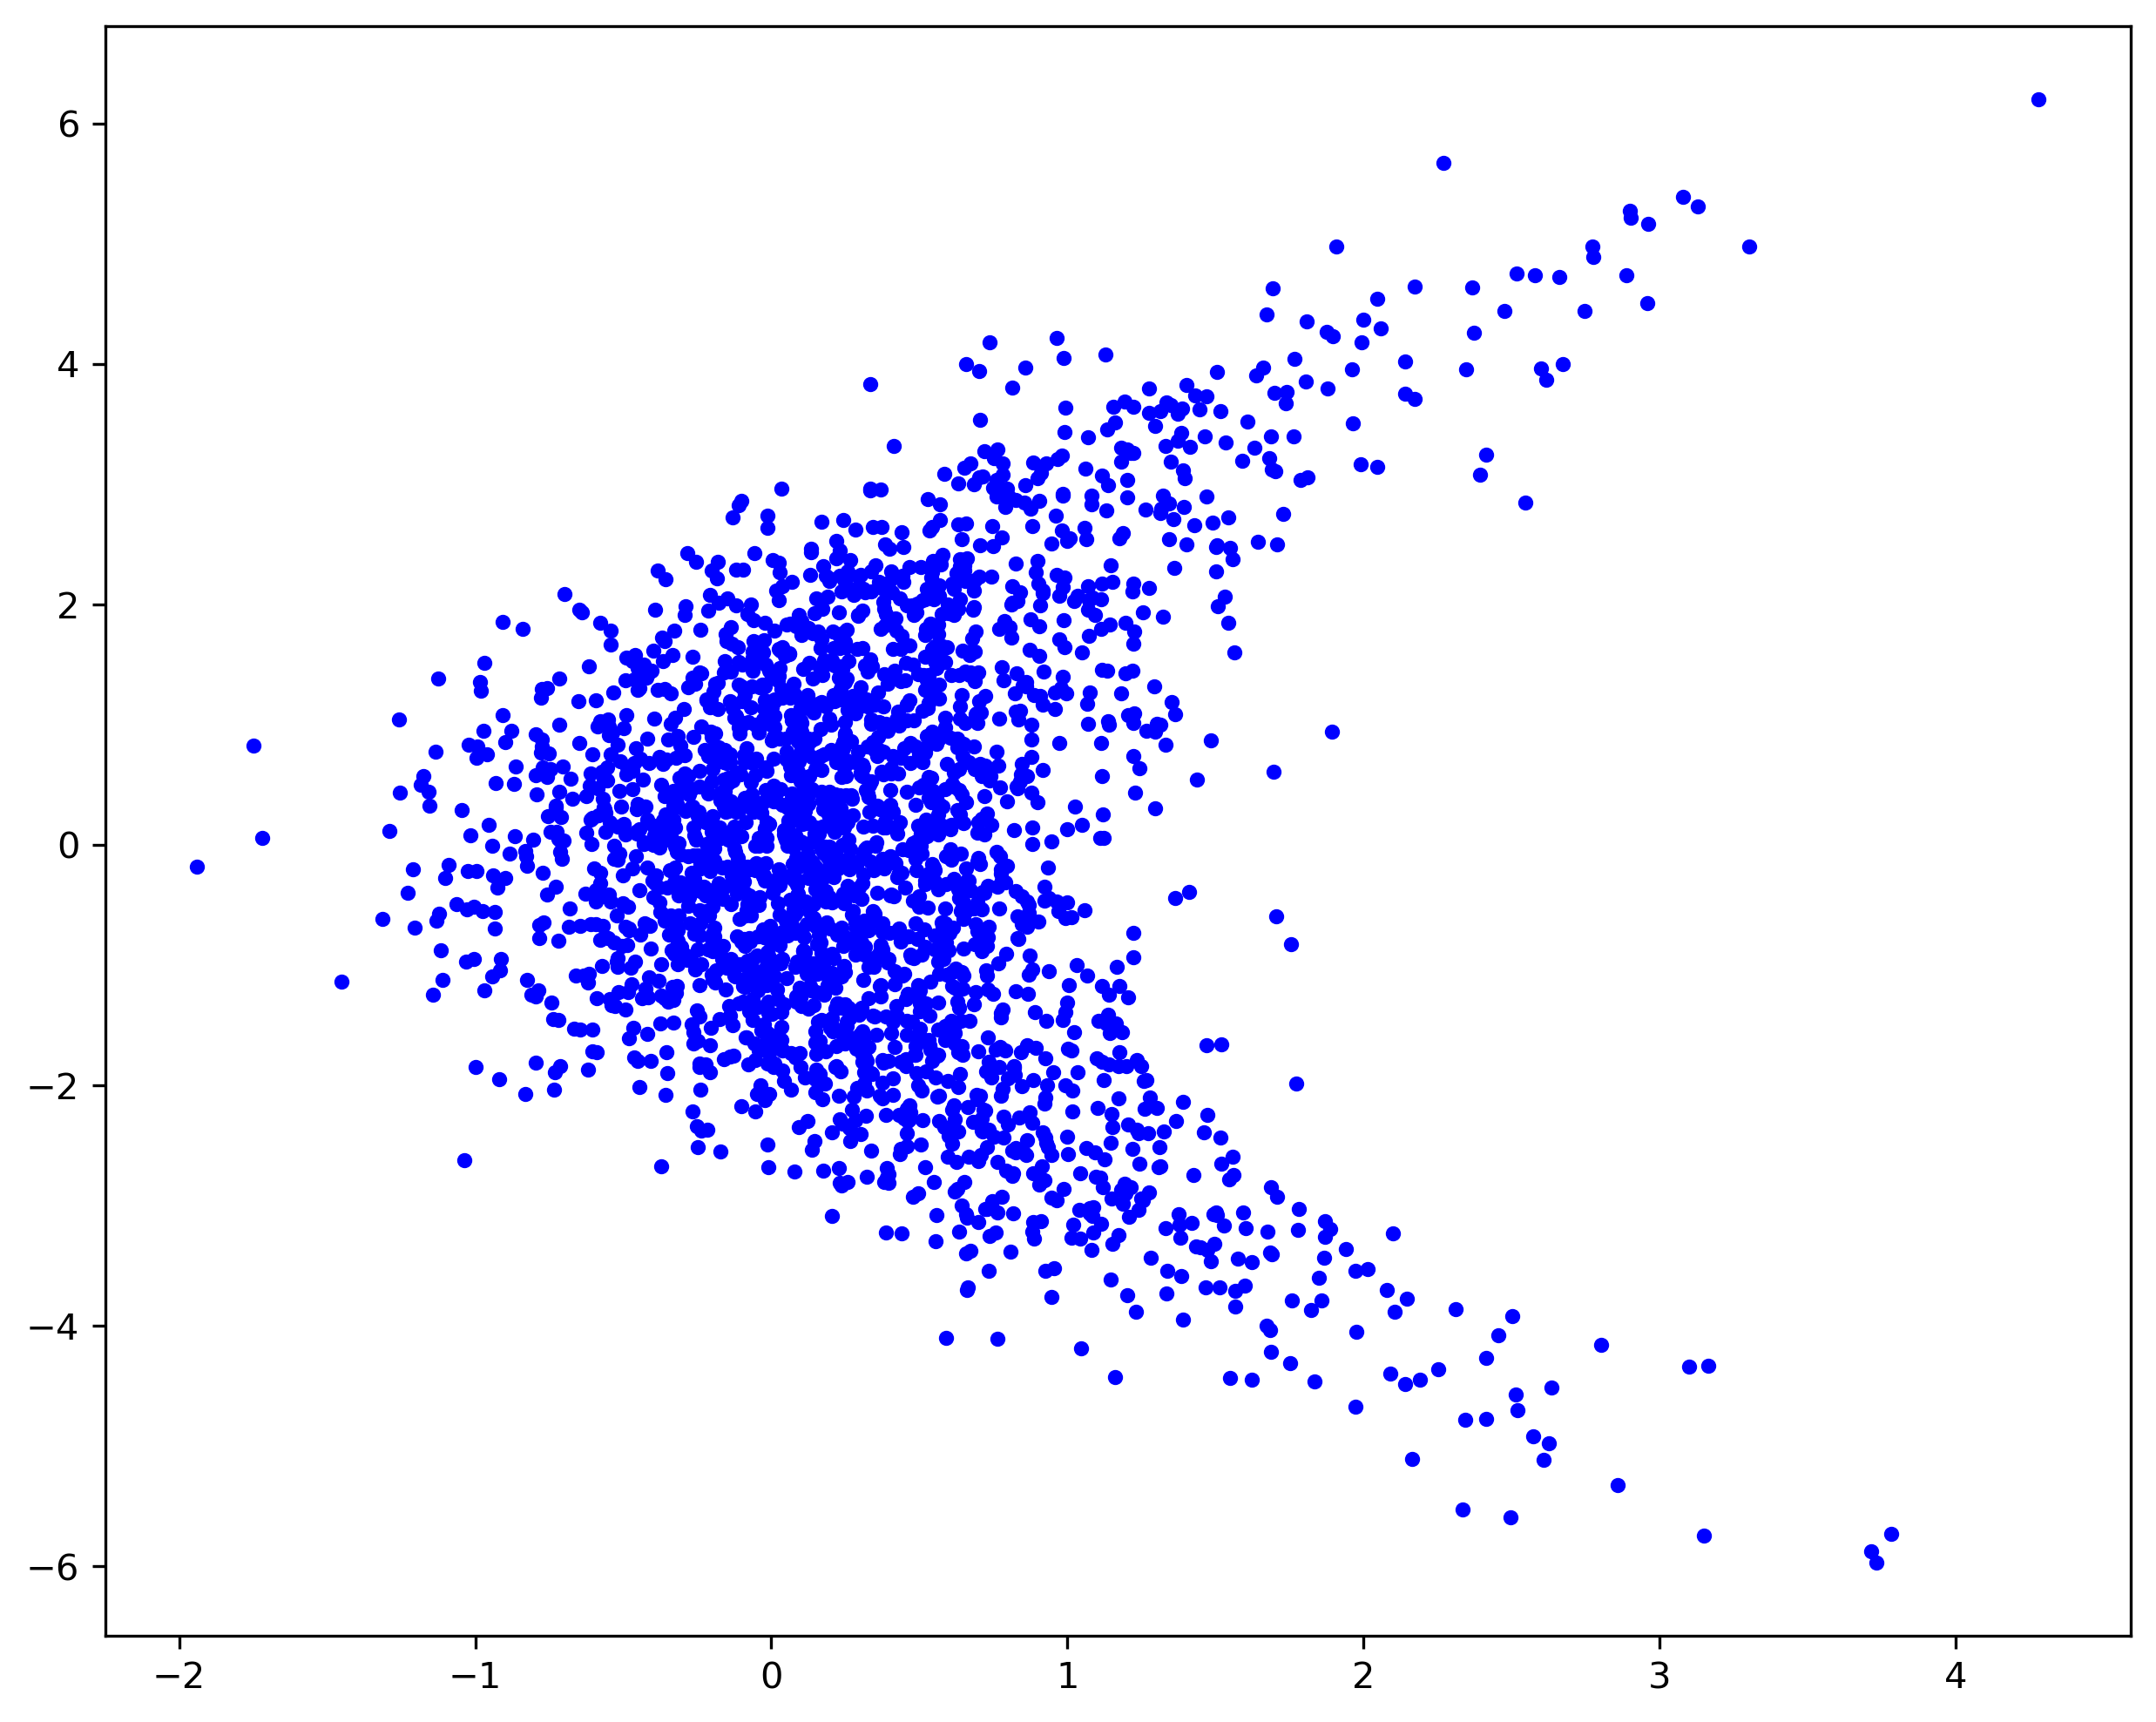
\includegraphics[width=\textwidth]{chapter5/results/visualisations/datasets/single_banana.png}
\caption{Single Banana}
\end{subfigure}
\begin{subfigure}[b]{0.32\textwidth}
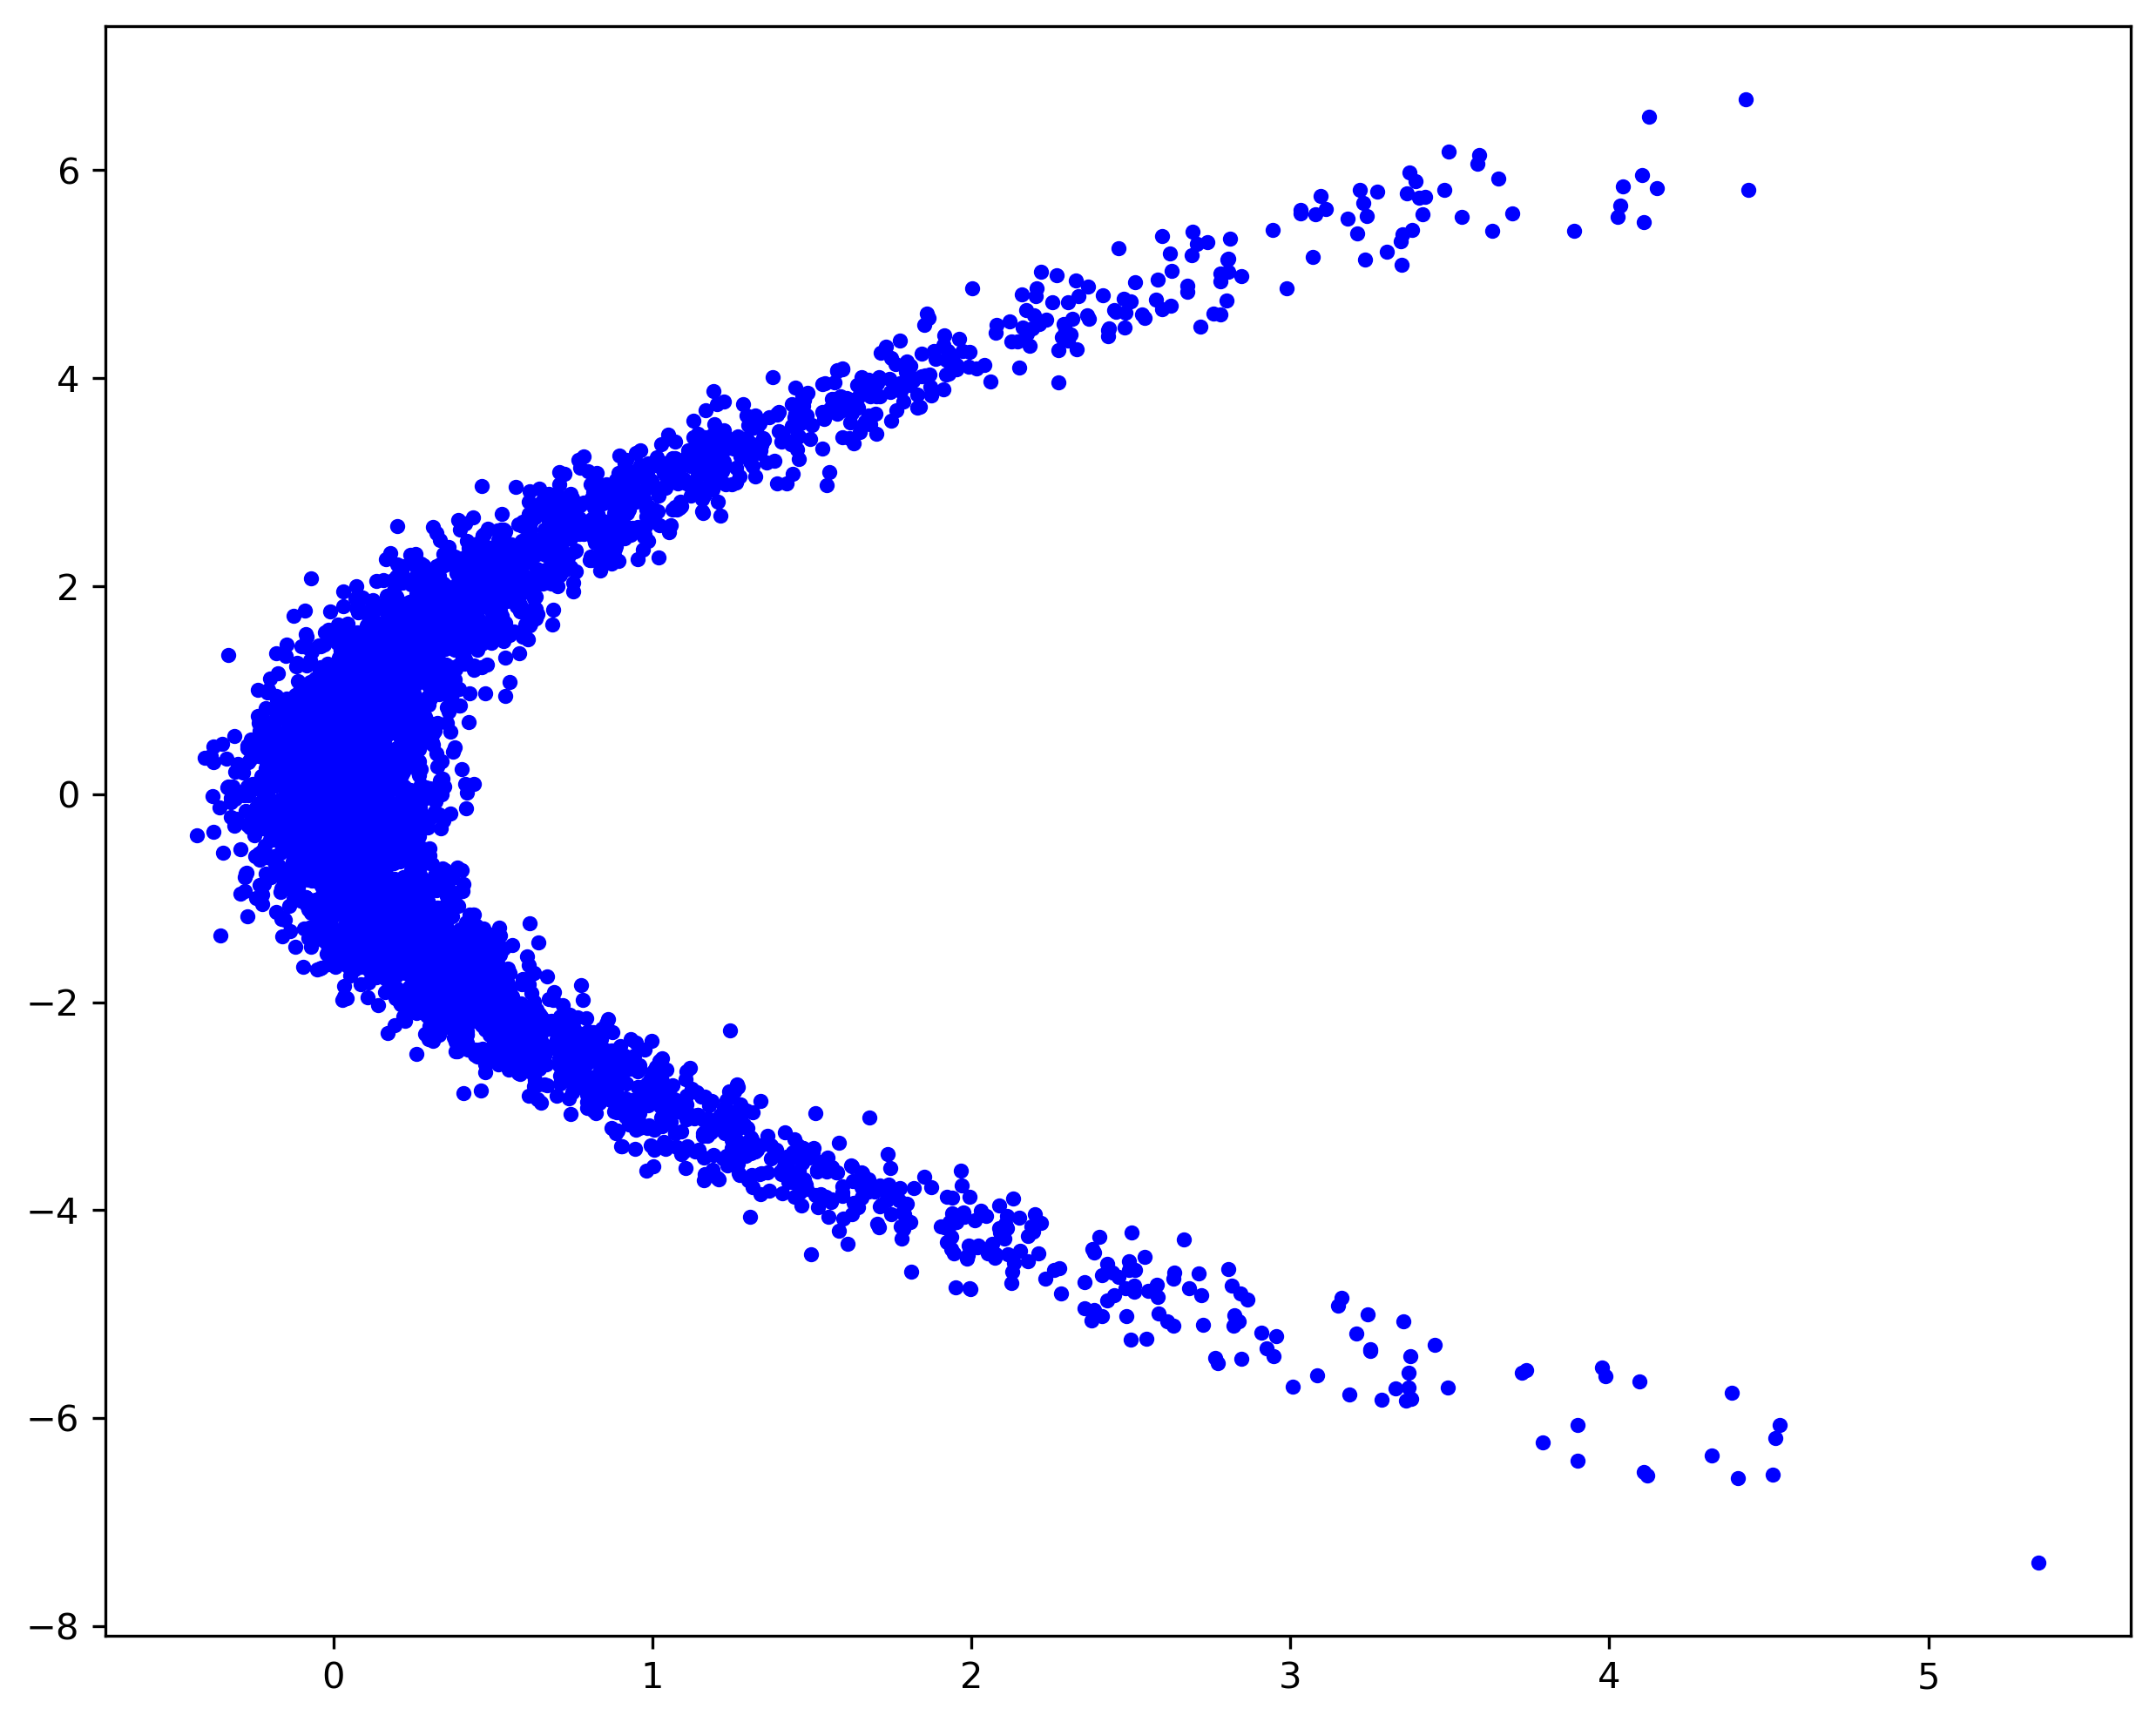
\includegraphics[width=\textwidth]{chapter5/results/visualisations/datasets/squeezed_single_banana.png}
\caption{Squeezed Single Banana}
\end{subfigure}
\begin{subfigure}[b]{0.32\textwidth}
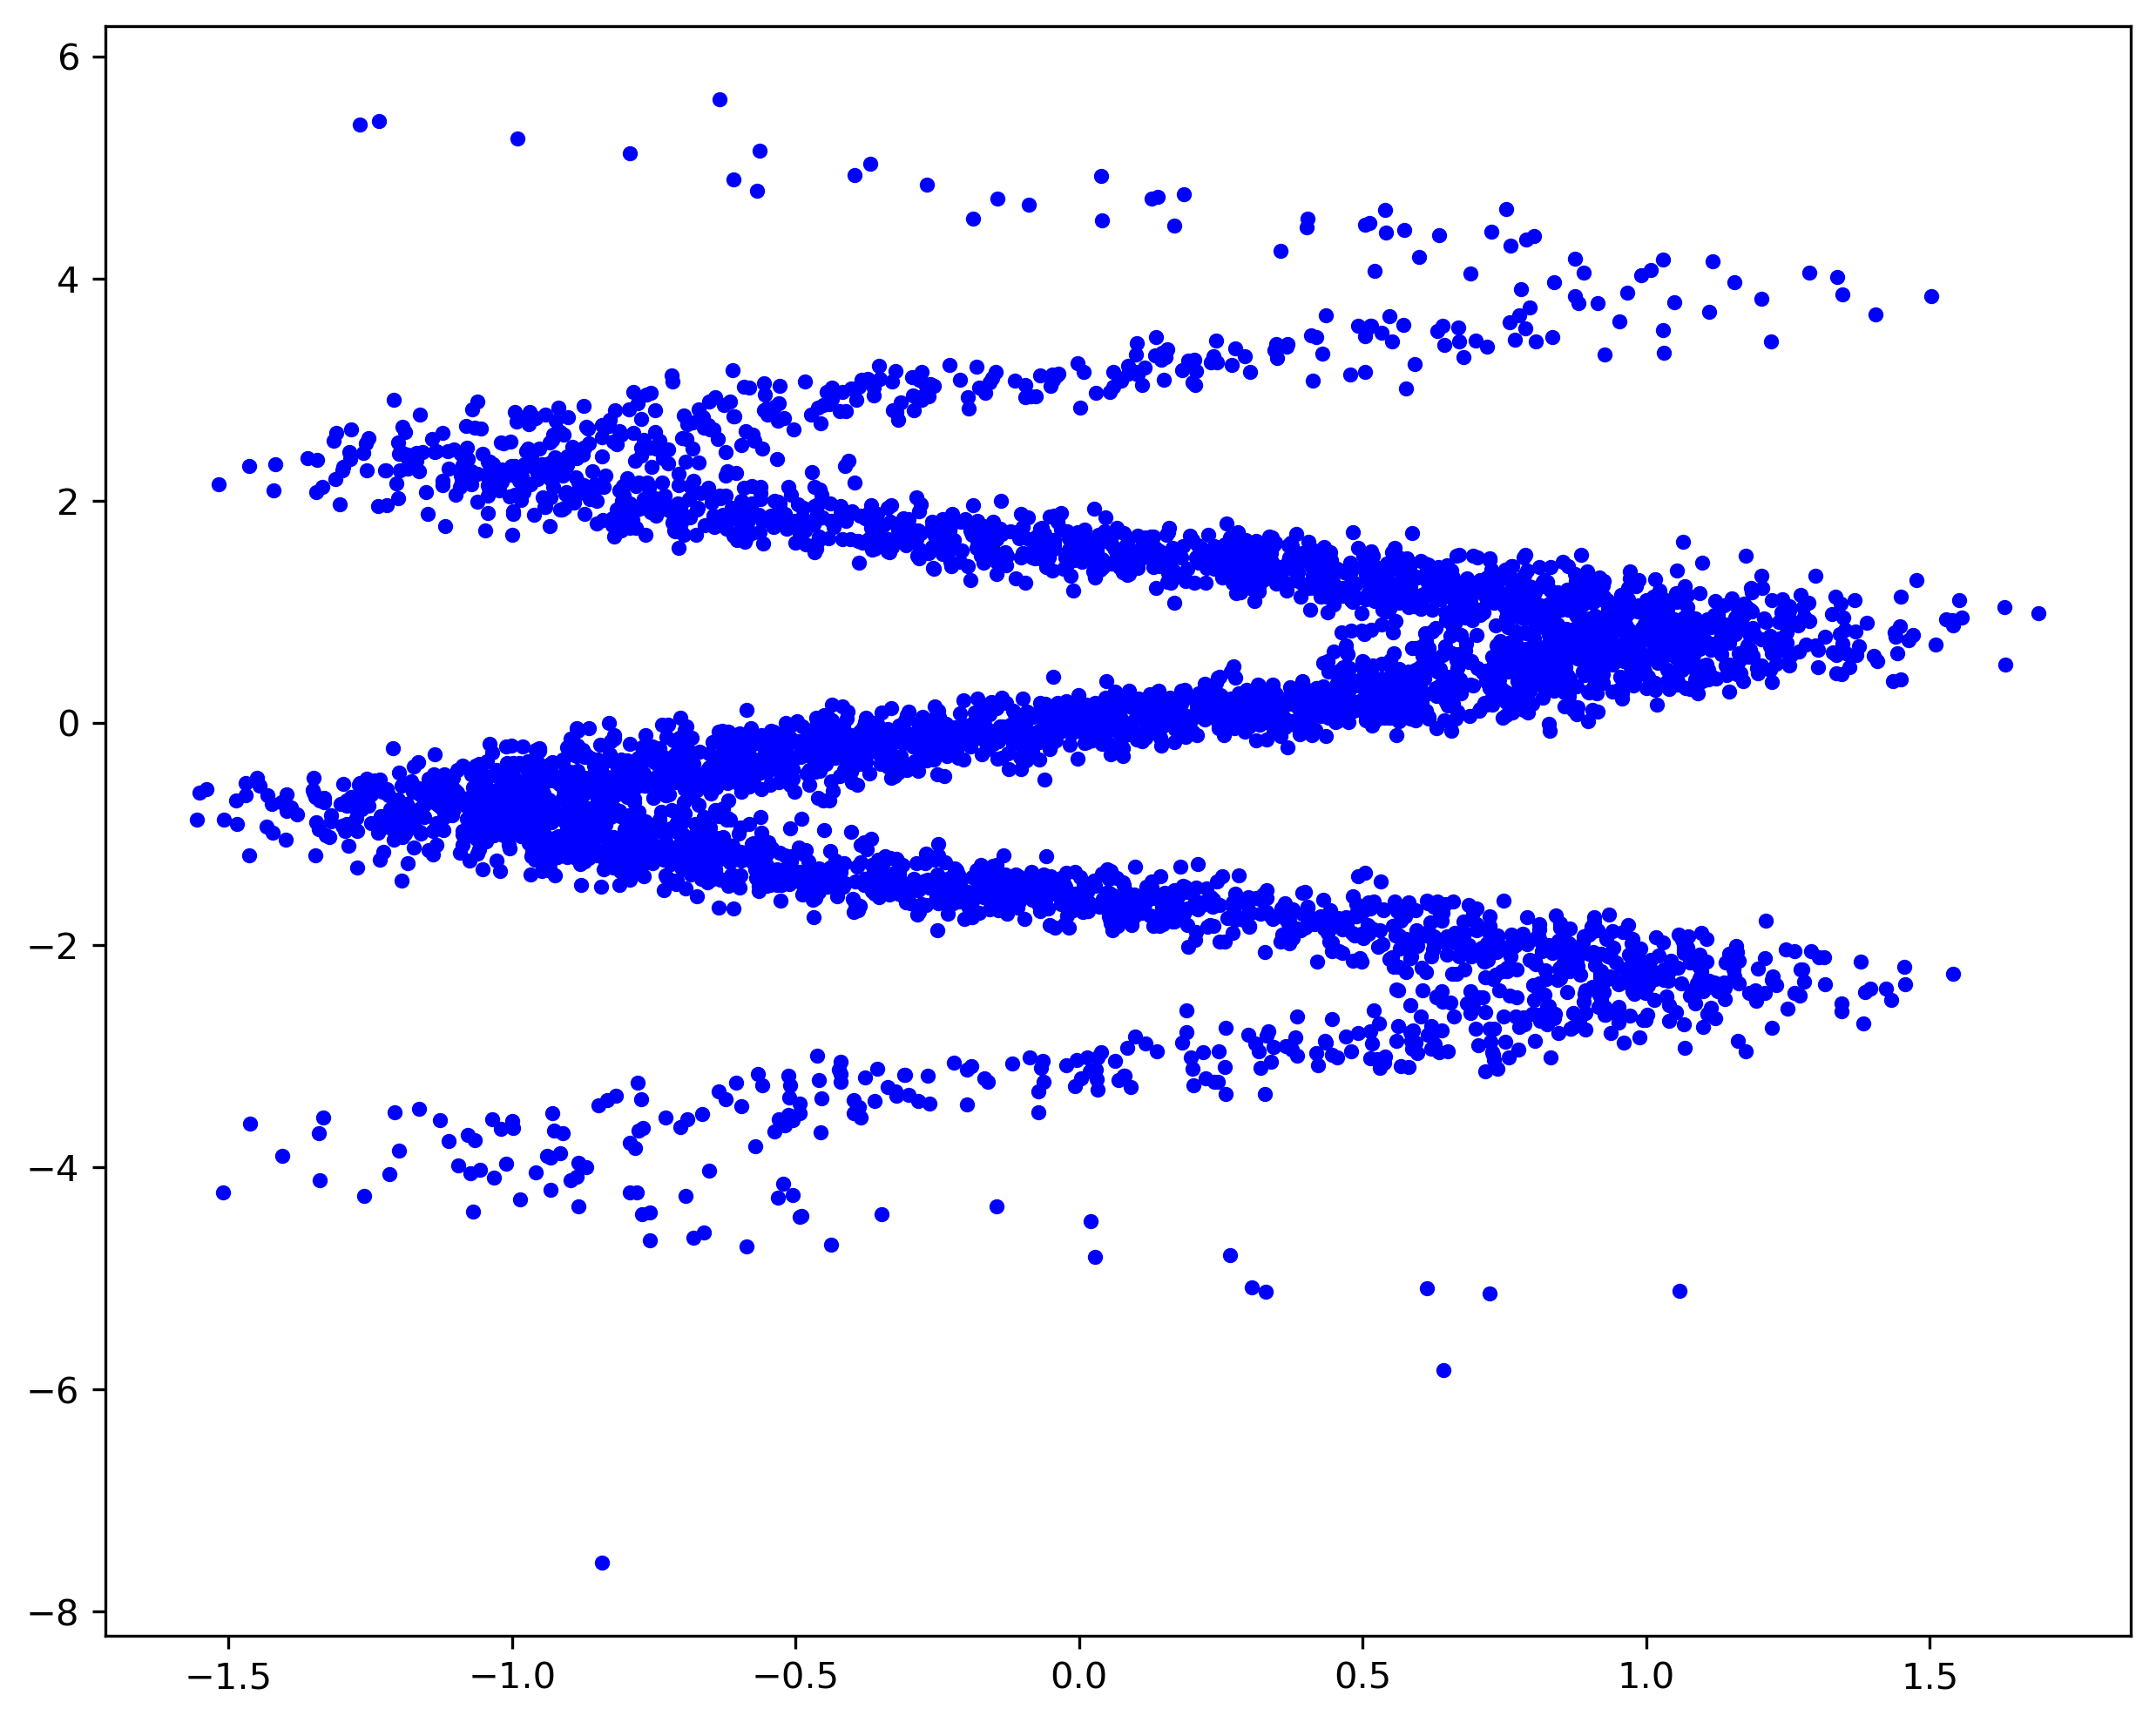
\includegraphics[width=\textwidth]{chapter5/results/visualisations/datasets/river.png}
\caption{River}
\end{subfigure}
\caption{Visualization of the datasets used in our manifold mapping experiments.}
\label{fig:datasets}
\end{figure}

In our manifold mapping experiments (\ref{sec:manifold-mappings-experiments}), we use the following datasets illustrated in \ref{fig:datasets}:

\begin{itemize}
    \item \textit{Single Banana Dataset}: A two-dimensional dataset shaped like a curved banana.
    \item \textit{Squeezed Single Banana Dataset}: A variant of the Single Banana with a tighter bend.
    \item \textit{River Dataset}: A more complex 2D dataset resembling the meandering path of a river.
\end{itemize}

Each dataset is constructed by defining specific diffeomorphisms $\diffeo$ and convex quadratic functions $\psi$, then sampling from the resulting probability density using Langevin Monte Carlo Markov Chain (MCMC) with Metropolis-Hastings correction. The probability density function is defined as:

\begin{equation}
    p(\mathbf{x}) \propto e^{-\psi(\diffeo(\mathbf{x}))},
    \label{eq:stroco-diffeo-density-ap}
\end{equation}

where the strongly convex function $\psi$ is given by:

\begin{equation}
    \psi(\mathbf{v}) = \frac{1}{2} \mathbf{v}^\top A^{-1} \mathbf{v},
    \label{eq:quadratic-stroco-ap}
\end{equation}

and $A$ is a positive-definite diagonal matrix. The specific choices of $\diffeo$ and $A$ for each dataset determine its geometric properties.

\subsubsection{Diffeomorphisms and Convex Quadratic Functions}

The key differences between the datasets arise from the diffeomorphism $\diffeo$ and the covariance matrix $\mathbf{A}$ used in the sampling process. Below, we describe the specific settings for each dataset.

\paragraph{1. Single Banana Dataset}

\begin{itemize}
    \item Diffeomorphism: 
    \[
    \diffeo(\mathbf{x}) = \begin{pmatrix} 
    x_1 - a x_2^2 - z \\
    x_2 
    \end{pmatrix}
    \]
    where $a = \frac{1}{9}$ and $z = 0$.
    \item Covariance matrix:
    \[
    \mathbf{A} = \begin{pmatrix} 
    \frac{1}{4} & 0 \\
    0 & 4 
    \end{pmatrix}
    \]
\end{itemize}

\paragraph{2. Squeezed Single Banana Dataset}

\begin{itemize}
    \item Diffeomorphism: Same as the Single Banana Dataset.
    \item Covariance matrix:
    \[
    \mathbf{A} = \begin{pmatrix} 
    \frac{1}{81} & 0 \\
    0 & 4 
    \end{pmatrix}
    \]
\end{itemize}

\paragraph{3. River Dataset}

\begin{itemize}
    \item Diffeomorphism: 
    \[
    \diffeo(\mathbf{x}) = \begin{pmatrix} 
    x_1 - \sin(a x_2) - z \\
    x_2 
    \end{pmatrix}
    \]
    where $a = 2$ and $z = 0$.
    \item Covariance matrix:
    \[
    \mathbf{A} = \begin{pmatrix} 
    \frac{1}{25} & 0 \\
    0 & 3 
    \end{pmatrix}
    \]
\end{itemize}

\subsubsection{Dataset Generation Algorithm}

Algorithm \ref{alg:Langevin MCMC with M-H correction} outlines the dataset generation process for all three datasets. The specific diffeomorphisms and quadratic functions differ for each dataset.

\begin{algorithm}[h]
\caption{General Dataset Generation Algorithm}
\label{alg:Langevin MCMC with M-H correction}
\begin{algorithmic}[1]
\REQUIRE Number of samples $N$, MCMC steps $T$, Step size $\delta$, Diffeomorphism $\diffeo$, Covariance matrix $\mathbf{\Lambda}$
\ENSURE Dataset $\{\mathbf{x}_1, \mathbf{x}_2, \dots, \mathbf{x}_N\}$
\STATE Initialize: Set initial state $\mathbf{x}_0 = \mathbf{0} \in \mathbb{R}^2$.
\FOR{$i = 1$ to $N$}
    \STATE $\mathbf{x} = \mathbf{x}_0$
    \FOR{$k = 1$ to $T$}
        \STATE Compute the score function $\nabla_{\mathbf{x}} \log p_{\text{target}}(\mathbf{x})$.
        \STATE Propose $\mathbf{x}' = \mathbf{x} + \frac{\delta^2}{2} \nabla_{\mathbf{x}} \log p_{\text{target}}(\mathbf{x}) + \delta \boldsymbol{\eta}$, where $\boldsymbol{\eta} \sim \mathcal{N}(\mathbf{0}, \mathbf{I}_2)$.
        
        \STATE Compute the forward kernel:
        \[
        K_{\text{forward}} = \frac{|\mathbf{x} - \mathbf{x}' + \frac{\delta^2}{2} \nabla_{\mathbf{x}'} \log p_{\text{target}}(\mathbf{x}')|^2}{2\delta^2}
        \]

        \STATE Compute the reverse kernel:
        \[
        K_{\text{reverse}} = \frac{|\mathbf{x}' - \mathbf{x} + \frac{\delta^2}{2} \nabla_{\mathbf{x}} \log p_{\text{target}}(\mathbf{x})|^2}{2\delta^2}
        \]
        
        \STATE Compute the Metropolis-Hastings acceptance probability:
        \[
        A = \min\left(1, \frac{p_{\text{target}}(\mathbf{x}')}{p_{\text{target}}(\mathbf{x})} \exp\left( -K_{\text{forward}} + K_{\text{reverse}} \right) \right)
        \]
        
        \STATE Accept $\mathbf{x}'$ with probability $A$; else set $\mathbf{x}' = \mathbf{x}$.
        \STATE Update $\mathbf{x} = \mathbf{x}'$.
    \ENDFOR
    \STATE Store the final $\mathbf{x}$ as sample $\mathbf{x}_i$.
\ENDFOR
\end{algorithmic}
\end{algorithm}

\subsection{Datasets for Riemannian Autoencoder Experiments}
\label{app:rae_datasets}

In the Riemannian autoencoder experiments (\ref{sec:RAE-experiments}), we use the following datasets:
\begin{itemize}
    \item \textit{Hemisphere}(\textit{d'}, \textit{d}) Dataset: Samples drawn from the upper hemisphere of a \textit{d'}-dimensional unit sphere and embedded into $\mathbb{R}^d$ via a random isometric mapping.
    \item \textit{Sinusoid}(\textit{d'}, \textit{d}) Dataset: Generated by applying sinusoidal transformations to \textit{d'}-dimensional latent variables, resulting in a complex, nonlinear manifold in $\mathbb{R}^d$.
\end{itemize}

\subsection{Hemisphere($d'$, $d$) Dataset}

The \textit{Hemisphere}($d'$, $d$) dataset consists of samples drawn from the upper hemisphere of a $d'$-dimensional unit sphere, which are then embedded into a $d$-dimensional ambient space using a random isometric embedding. Below are the steps involved in constructing this dataset.

\paragraph{1. Sampling from the Upper Hemisphere}

We begin by sampling points from the upper hemisphere of the $d'$-dimensional unit sphere $S^{d'}_+ \subset \mathbb{R}^{d'+1}$. The upper hemisphere is defined as:
\[
S^{d'}_+ = \left\{ \mathbf{x} \in \mathbb{R}^{d'+1} : \|\mathbf{x}\| = 1, \, x_1 \geq 0 \right\}.
\]
The first angular coordinate $\theta_1$ is sampled from a Beta distribution with shape parameters $\alpha = 5$ and $\beta = 5$, scaled to the interval $\left[ 0, \frac{\pi}{2} \right]$. This sampling method emphasizes points near the ``equator'' of the hemisphere. The remaining angular coordinates $\theta_2, \ldots, \theta_{d'}$ are sampled uniformly from the interval $\left[ 0, \pi \right]$:
\[
\theta_1 \sim \text{Beta}(5, 5) \cdot \left( \frac{\pi}{2} \right), \quad \theta_i \sim \text{Uniform}(0, \pi), \, \text{for } i = 2, \ldots, d'.
\]

\paragraph{2. Conversion to Cartesian Coordinates}

Next, each sampled point in spherical coordinates is converted into Cartesian coordinates in $\mathbb{R}^{d'+1}$ using the following transformation equations:
\[
x_1 = \cos(\theta_1), \quad x_2 = \sin(\theta_1) \cos(\theta_2), \quad \dots, \quad x_{d'+1} = \sin(\theta_1) \sin(\theta_2) \cdots \sin(\theta_{d'}).
\]
This conversion ensures that the sampled points lie on the surface of the unit sphere in $(d'+1)$-dimensional space.

\paragraph{3. Random Isometric Embedding into $\mathbb{R}^d$}

After sampling points on the hemisphere in $\mathbb{R}^{d'+1}$, the points are embedded into a $d$-dimensional ambient space ($d \geq d'+1$) using a random isometric embedding. The embedding process is as follows:

\begin{enumerate}
    \item Generate a random matrix $\mathbf{A} \in \mathbb{R}^{d \times (d'+1)}$, where each entry is sampled from a standard normal distribution $\mathcal{N}(0, 1)$.
    \item Perform a QR decomposition on matrix $\mathbf{A}$ to obtain $\mathbf{Q} \in \mathbb{R}^{d \times (d'+1)}$:
    \[
    \mathbf{A} = \mathbf{Q} \mathbf{R}.
    \]
    The columns of \( \mathbf{Q} \) form an orthonormal basis for a \((d'+1)\)-dimensional subspace of \( \mathbb{R}^d \), ensuring that \( \mathbf{Q} \) defines an isometric embedding from \( \mathbb{R}^{d'+1} \) into \( \mathbb{R}^d \). This guarantees that distances and angles are preserved during the mapping, maintaining the geometric structure of the original space within the higher-dimensional ambient space.

    \item Use matrix $\mathbf{Q}$ to map each sample $\mathbf{x} \in \mathbb{R}^{d'+1}$ into the ambient space:
    \[
    \mathbf{y} = \mathbf{Q}\mathbf{x},
    \]
    where $\mathbf{y} \in \mathbb{R}^d$ are the embedded samples.
\end{enumerate}

\begin{algorithm}
    \caption{Hemisphere($d'$, $d$) Dataset Generation}
    \begin{algorithmic}[1]
        \STATE \textbf{Input:} Intrinsic dimension $d'$, ambient dimension $d$, number of samples $n$, Beta distribution parameters $\alpha = 5$, $\beta = 5$
        \STATE \textbf{Output:} Dataset $\mathbf{Y} \in \mathbb{R}^{n \times d}$

        \STATE \textbf{Step 1: Generate Random Isometric Embedding}
        \STATE Generate a random matrix $\mathbf{A} \in \mathbb{R}^{d \times (d'+1)}$ with entries from $\mathcal{N}(0, 1)$
        \STATE Perform QR decomposition on $\mathbf{A}$ to obtain $\mathbf{Q} \in \mathbb{R}^{d \times (d'+1)}$:
        \[
        \mathbf{A} = \mathbf{Q} \mathbf{R}
        \]

        \STATE \textbf{Step 2: Construct Dataset}
        \FOR{$i = 1$ to $n$}
            \STATE \textbf{Step 2.1: Sample Spherical Coordinates}
            \STATE Sample the first angular coordinate $\theta_1$ from a scaled Beta distribution:
            \[
            \theta_1 \sim \text{Beta}(\alpha, \beta) \cdot \left( \frac{\pi}{2} \right)
            \]
            \STATE Sample the remaining angular coordinates $\theta_2, \dots, \theta_{d'}$ from a uniform distribution:
            \[
            \theta_i \sim \text{Uniform}(0, \pi), \quad \text{for } i = 2, \dots, d'
            \]

            \STATE \textbf{Step 2.2: Convert to Cartesian Coordinates}
            \STATE Convert the spherical coordinates to Cartesian coordinates $\mathbf{x}_i \in \mathbb{R}^{d'+1}$ using:
            \[
            x_1 = \cos(\theta_1), \quad x_2 = \sin(\theta_1) \cos(\theta_2), \dots, \quad x_{d'+1} = \sin(\theta_1) \sin(\theta_2) \cdots \sin(\theta_{d'}).
            \]

            \STATE \textbf{Step 2.3: Embed Sample $\mathbf{x}_i$ into Ambient Space}
            \STATE Map the sample $\mathbf{x}_i$ to the ambient space using:
            \[
            \mathbf{y}_i = \mathbf{Q} \mathbf{x}_i
            \]

            \STATE Append $\mathbf{y}_i$ to the dataset $\mathbf{Y}$
        \ENDFOR
        
        \STATE \textbf{Return:} The final dataset $\mathbf{Y} = [\mathbf{y}_1, \mathbf{y}_2, \dots, \mathbf{y}_n]$
    \end{algorithmic}
\end{algorithm}

\subsection{Sinusoid($d'$, $d$) Dataset}

The \textit{Sinusoid}($d'$, $d$) dataset represents a $d'$-dimensional manifold embedded in $d$-dimensional space through nonlinear sinusoidal transformations. Below are the detailed steps involved in constructing this dataset.

\paragraph{1. Sampling Latent Variables}

The latent variables $\mathbf{z} \in \mathbb{R}^{d'}$ are sampled from a multivariate Gaussian distribution with zero mean and isotropic variance, as follows:
\[
\mathbf{z} \sim \mathcal{N}\left( 0, \sigma_m^2 I_{d'} \right),
\]
where $\sigma_m^2$ controls the variance along each intrinsic dimension, and $I_{d'}$ is the $d' \times d'$ identity matrix. The value of $\sigma_m^2$ is set to 3 for our experiments.

\paragraph{2. Defining Ambient Coordinates with Sinusoidal Transformations}

For each of the $d-d'$ ambient dimensions, we construct a shear vector \( \mathbf{a}_j \in \mathbb{R}^{d'} \), with its elements drawn uniformly from the interval \([1, 2]\):
\[
\mathbf{a}_j \sim \text{Uniform}(1, 2)^{d'}, \quad \text{for } j = 1, \dots, d-d'.
\]

The shear vectors \( \mathbf{a}_j \) apply a fixed linear transformation to the latent space \( \mathbf{z} \in \mathbb{R}^{d'} \), determining how the latent variables influence each ambient dimension. These vectors, sampled once for each of the $d-d'$ ambient dimensions, modulate the scale and periodicity of the sinusoidal transformation.

Each ambient coordinate \( x_j \) is generated as a sinusoidal function of the inner product between \( \mathbf{a}_j \) and \( \mathbf{z} \), with a small Gaussian noise added for regularization.

\[
x_j = \sin\left( \mathbf{a}_j^\top \mathbf{z} \right) + \epsilon_j,
\]
where \( \epsilon_j \sim \mathcal{N}(0, \sigma_a^2) \) is Gaussian noise with variance \( \sigma_a^2 \). In our experiments, we set \( \sigma_a^2 = 10^{-3} \).

\paragraph{3. Constructing the Dataset Samples}

The final samples $\mathbf{y} \in \mathbb{R}^d$ are formed by concatenating the ambient coordinates $x_1, x_2, \dots, x_{d-d'}$ with the latent variables $z_1, z_2, \dots, z_{d'}$:
\[
\mathbf{y} = \left[ x_1, x_2, \dots, x_{d-d'}, \, z_1, z_2, \dots, z_{d'} \right]^\top.
\]

\begin{algorithm}
    \caption{Sinusoid($d'$, $d$) Dataset Generation}
    \begin{algorithmic}[1]
        \STATE \textbf{Input:} Intrinsic dimension $d'$, ambient dimension $d$, number of samples $n$, variance $\sigma_m^2 = 3$, noise variance $\sigma_a^2 = 10^{-3}$
        \STATE \textbf{Output:} Dataset $\mathbf{Y} \in \mathbb{R}^{n \times d}$

        \STATE \textbf{Step 1: Generate Shear Vectors}
        \FOR{$j = 1$ to $d - d'$}
            \STATE Sample shear vector $\mathbf{a}_j \in \mathbb{R}^{d'}$ from \text{Uniform}$(1, 2)^{d'}$
        \ENDFOR

        \STATE \textbf{Step 2: Construct Dataset}
        \FOR{$i = 1$ to $n$}
            \STATE \textbf{Step 2.1: Sample Latent Variables}
            \STATE Generate latent variables $\mathbf{z}_i \in \mathbb{R}^{d'}$ from a multivariate Gaussian:
            \[
            \mathbf{z}_i \sim \mathcal{N}(0, \sigma_m^2 \cdot I_{d'})
            \]

            \STATE \textbf{Step 2.2: Compute Ambient Coordinates for Sample $i$}
            \FOR{$j = 1$ to $d - d'$}
                \STATE Compute ambient coordinate $x_j$ for the $i$-th sample:
                \[
                x_j = \sin\left( \mathbf{a}_j^\top \mathbf{z}_i \right) + \epsilon_j, \quad \epsilon_j \sim \mathcal{N}(0, \sigma_a^2)
                \]
            \ENDFOR

            \STATE \textbf{Step 2.3: Form Final Sample $\mathbf{y}_i$}
            \STATE Concatenate the ambient coordinates $\mathbf{x} = [x_1, x_2, \dots, x_{d-d'}]$ and the latent variables $\mathbf{z}_i$ to form the final sample $\mathbf{y}_i \in \mathbb{R}^d$:
            \[
            \mathbf{y}_i = [x_1, x_2, \dots, x_{d-d'}, z_1, z_2, \dots, z_{d'}]^\top
            \]

            \STATE Append $\mathbf{y}_i$ to the dataset $\mathbf{Y}$
        \ENDFOR
        
        \STATE \textbf{Return:} The final dataset $\mathbf{Y} = [\mathbf{y}_1, \mathbf{y}_2, \dots, \mathbf{y}_n]$
    \end{algorithmic}
\end{algorithm}

\section{Error Metrics for Evaluation of Pullback Geometries}
\label{app:Error metrics for evaluation of Pullback Geometries}

\paragraph{Geodesic Error.}
The geodesic error measures the difference between geodesics on the learned and ground truth pullback manifolds. Given two points \(\mathbf{x}_0, \mathbf{x}_1 \in \mathbb{R}^{\dimInd}\), let \(\gamma_{\mathbf{x}_0, \mathbf{x}_1}^{\diffeo_{\theta_2}}(t)\) and \(\gamma_{\mathbf{x}_0, \mathbf{x}_1}^{\diffeo_{\mathrm{GT}}}(t)\) denote the geodesics induced by the learned map \(\diffeo_{\theta_2}\) and the ground truth map \(\diffeo_{\mathrm{GT}}\), respectively, where \(t \in [0, 1]\).

The geodesic error is calculated as the mean Euclidean distance between the learned and ground truth geodesics over \(N\) pairs of points:

\[
\text{Geodesic Error} = \frac{1}{N} \sum_{i=1}^{N} \frac{1}{T} \sum_{k=1}^{T} \left\| \gamma_{\mathbf{x}_0^{(i)}, \mathbf{x}_1^{(i)}}^{\diffeo_{\theta_2}}(t_k) - \gamma_{\mathbf{x}_0^{(i)}, \mathbf{x}_1^{(i)}}^{\diffeo_{\mathrm{GT}}}(t_k) \right\|_2,
\]
where \(T\) is the number of time steps used to discretize the geodesic, and \(t_k = \frac{k-1}{T-1}\) for \(k = 1, \dots, T\).

This metric captures the average discrepancy between the learned and ground truth geodesics, reflecting the accuracy of the learned pullback manifold.

\paragraph{Variation Error.}
The variation error quantifies the sensitivity of the geodesic computation under small perturbations to one of the endpoints. For two points \(\mathbf{x}_0, \mathbf{x}_1 \in \mathbb{R}^{\dimInd}\), let \(\mathbf{z} = \mathbf{x}_1 + \Delta\mathbf{x}\), where \(\Delta\mathbf{x}\) is a small perturbation applied to \(\mathbf{x}_1\). Define \(\gamma_{\mathbf{x}_0, \mathbf{x}_1}^{\diffeo_{\theta_2}}(t)\) and \(\gamma_{\mathbf{x}_0, \mathbf{z}}^{\diffeo_{\theta_2}}(t)\) as the geodesics from \(\mathbf{x}_0\) to \(\mathbf{x}_1\) and \(\mathbf{z}\), respectively, induced by the learned map \(\diffeo_{\theta_2}\).

The variation error is calculated as the mean Euclidean distance between the geodesic from \(\mathbf{x}_0\) to \(\mathbf{x}_1\) and the perturbed geodesic from \(\mathbf{x}_0\) to \(\mathbf{z}\):

\[
\text{Variation Error} = \frac{1}{N} \sum_{i=1}^{N} \frac{1}{T} \sum_{k=1}^{T} \left\| \gamma_{\mathbf{x}_0^{(i)}, \mathbf{x}_1^{(i)}}^{\diffeo_{\theta_2}}(t_k) - \gamma_{\mathbf{x}_0^{(i)}, \mathbf{z}^{(i)}}^{\diffeo_{\theta_2}}(t_k) \right\|_2,
\]
where \(N\) is the number of sampled point pairs, \(T\) is the number of time steps used to discretize the geodesic, and \(t_k = \frac{k-1}{T-1}\) for \(k = 1, \dots, T\).

This metric evaluates the robustness of the learned geodesic against small perturbations, providing insight into the stability of the learned manifold.

\section{Training Details}
\label{app:training_details}

The following section describes the important configuration parameters for reproducing the experiments on manifold mappings. All experiments share some common parameters, which are listed below, while dataset-specific parameters are provided in Table~\ref{tab:training_details}.

\textbf{Common Parameters:}
\begin{itemize}
    \item \textbf{Optimizer:} Adam with \texttt{betas} = (0.9, 0.99), \texttt{eps} = $1 \times 10^{-8}$, and weight decay of $1 \times 10^{-5}$.
    \item \textbf{Learning Rate Schedule:} Warm-up cosine annealing with 1000 warm-up steps.
    \item \textbf{Gradient Clipping:} Gradient norm clipped to 1.0.
    \item \textbf{Model Architecture:} A composition of affine coupling layers is used, where each layer transforms part of the input while keeping the other part unchanged. The transformation function in each layer is modeled by a residual network (ResNet) consisting of 64 hidden features, 2 residual blocks, ReLU activations, and no batch normalization. Dropout is set to 0, and transformations alternate across different dimensions at each layer.
\end{itemize}

\begin{table}[htbp]
    \centering
    \caption{Training configurations for each experiment.}
    \label{tab:training_details}
    \begin{tabular}{|l|c|c|c|c|c|c|}
        \hline
        \textbf{Dataset} & \textbf{Flow Steps} & \textbf{Epochs} & \textbf{Batch Size} & $\lambda_{\text{iso}}$ & $\lambda_{\text{vol}}$ & \textbf{Learning Rate} \\
        \hline
        Sinusoid(1,3)     & 8  & 1000  & 64  & 1.0  & 1.0  & $3 \times 10^{-4}$ \\
        Sinusoid(2,3)     & 8  & 1000  & 64  & 1.0  & 1.0  & $3 \times 10^{-4}$ \\
        Sinusoid(5,20)    & 24 & 2000  & 128 & 1.2  & 2.5  & $4 \times 10^{-4}$ \\
        Hemisphere(2,3)   & 8  & 2000  & 64  & 1.0  & 1.0  & $4 \times 10^{-4}$ \\
        Hemisphere(5,20)  & 12 & 2000  & 64  & 0.75 & 1.2  & $4 \times 10^{-4}$ \\
        \hline
    \end{tabular}
\end{table}

\section{Data Manifold Approximation}
\label{app:data_manifold_approximation}

The learned manifold, shown in orange in \ref{fig:learned_charts}, is the set \( D_{\epsilon}(\mathcal{U}) \), where \( D_{\epsilon} \) is the RAE decoder \ref{eq:rae-decoder}, the set \( \mathcal{U} \) in the latent space is the open set given by
% Mathematically, let \( \manifold \subset \mathbb{R}^\dimInd \) represent the manifold embedded in the ambient space, and let \( \mathcal{U} \) be an open subset of \( \mathbb{R}^{d_{\epsilon}} \), defined as:
\[
    \mathcal{U} = \prod_{i=1}^{d_{\epsilon}} (-3\sqrt{\spdMatrixDiag_{\coordIndA_\sumIndA}}, 3\sqrt{\spdMatrixDiag_{\coordIndA_\sumIndA}})
\]
and \( \spdMatrixDiag_{\coordIndA_1}, \dots, \spdMatrixDiag_{\coordIndA_{d_{\epsilon}}} \) are the \( d_{\epsilon} \) highest learned variances corresponding to the ones used in the RAE construction. 

To visualize this in practice, we construct a mesh grid by linearly sampling each latent dimension from \( -3\sqrt{\spdMatrixDiag_{\coordIndA_\sumIndA}} \) to \( +3\sqrt{\spdMatrixDiag_{\coordIndA_\sumIndA}} \), for \( i = 1, \dots, d_{\epsilon} \), where \( d_{\epsilon} \) is the number of significant latent dimensions. Practically, the off-manifold latent dimensions (those corresponding to negligible variances) are set to zero. The decoder \( D_{\epsilon} \) then maps this grid from \( \mathcal{U} \) back to \( \mathbb{R}^\dimInd \), generating an approximation of the data manifold, as illustrated in \ref{fig:learned_charts}.


